\chapter{Interactions of ions with phospholipid membranes}
\label{chap:results}

Biological membranes naturally exist in a weak electrolytic solution of \ce{KCl} on the intracellular side, and of \ce{NaCl} on the extracellular side. 
The biological relevance of these ions reaches from relatively simple osmotic effects to the complex processes in neural signalling. 

Calcium is an important cation in biology, 
which takes part in many signalling pathways, e.g. triggering of the release of neurotransmitter in neurons,
and processes such as regulating cardiac rythm in heart. 
The interaction of \ce{Ca^{2+}} with phospholipid membranes has recieved attention recently from both experiments and simulations \citep{melcrova16, javanainen17}.

In the previous chapter, we presented new classical MD models of phospholipids,
which account for electrionic polarization via ECC (introduced in section~\ref{section:ecc}). 
It was demonstrated that such models, termed ECC-lipids, 
meet current accuracy standards in the field 
by comparing them with NMR order parameters and X-ray diffraction data (section~\ref{section:ecc-lipids}. 

In this chapter, we will provide detailed insight into the interactions of these ions with neutral and negatively charged model membranes,
namely with a POPC bilayer and to a bilayer with a composition of 5~POPC:1~POPS. 
We employ our newly developed models of ions and phospholipids, 
ECC-ions \citep{martinek17, kohagen16, Pluharova2014} and ECC-lipids \citep{melcr18}, 
which excel any state-of-the-art model of ions or lipids. 

First, we summarize the literature knowledge on the interactions of ions with membranes in experiments and simulations.
Then we demonstrate the outstanding accuracy of the newly developed model of POPC, ECC-POPC, 
in the responses of the head group order parameters.
The simulation study with a cationic surfactant 
validates ECC-POPC as an accurate model of the lipid electrometer concept observed in NMR experimnents. 
At last, we will provide detailed insight into the binding of cations to the neutral and negatively charged bilayers. 
We put extra stress on the interactions with \ce{Ca^{2+}}, 
for which we present the first simulation results that are in \emph{quantitative} agreement with experiments. \citep{catte16, melcr18}





\section{Lipid electrometer and binding of cations to phospholipid bilayers in experiments and simulations}
\label{section:electrometer_exp_sim} 

\textbf{ Recap the main outcomes of the NMRLipids II paper \citep{catte16}. }
Then introduce/continue with how to fix it. 
Include 1-2 figures. 

\textbf{ Recap the main outcomes of the NMRLipids IV paper. }
Prepare ground for the work-in-progress POPS model. 

\textbf{Electronic polarization is required for accurate head group response to membrane-bound charge in simulation. ECC-POPC paper text follows \dots  }

\begin{figure}[tb!] 
  \centering 
  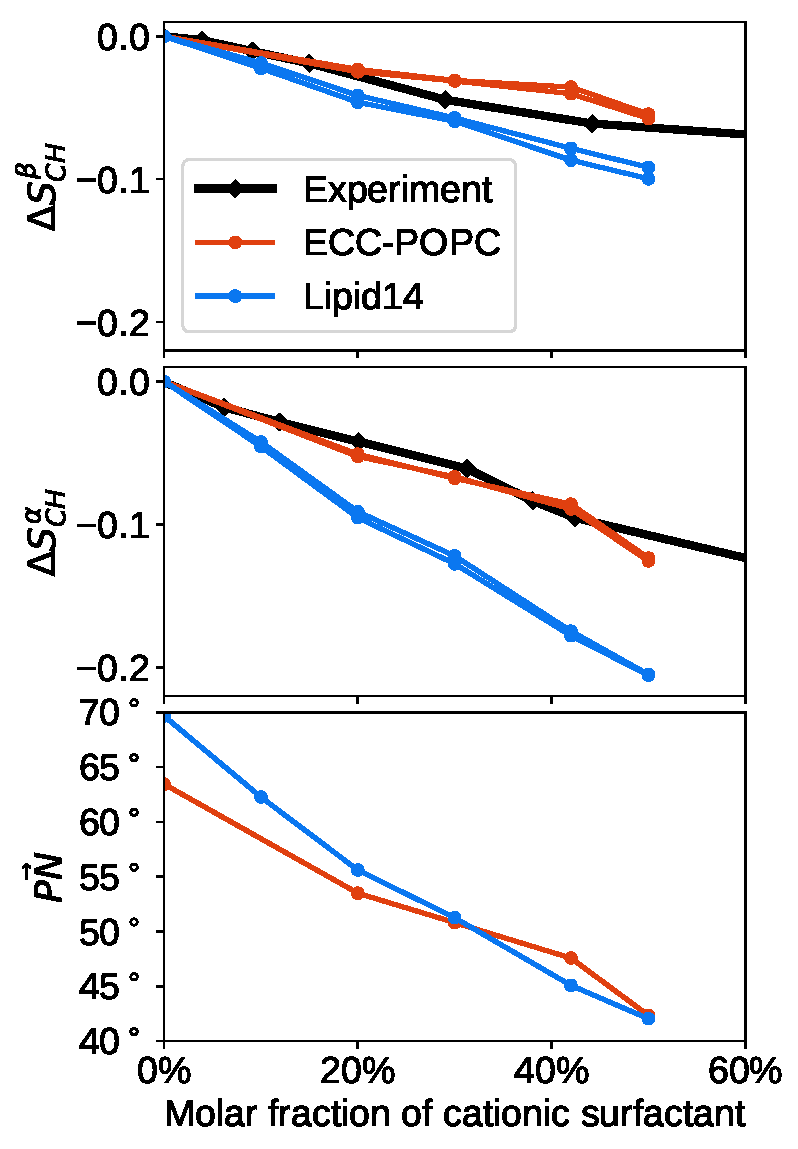
\includegraphics[width=8.0cm]{../img/ecc_popc/PN_angle_OrdPars-A-B_L14-ECCL17_q80_sig89_surf.pdf} 
  \caption{\label{OrderParameterCHANGESsurf} 
    The changes of head group order parameters and P-N vector orientation as a function of 
    a molar fraction of the cationic surfactant dihexadecyldimethylammonium in a POPC bilayer 
    from simulations and experiments \citep{scherer89} at 313 K.
  } 
\end{figure} 
 
The calibration of the response of the lipid electrometer to the amount of bound charge 
is measured for mixtures of POPC with monovalent cationic surfactants \citep{scherer89}.
In this work, we have chosen dihexadecyldimethylammonium. 
The amount of bound charge per PC 
in such systems is simply given by the molar fraction of the cationic surfactants, 
as essentially all of the surfactants locate to the lipid bilayers 
due to the two long hydrophobic tails.
The NMR measurements of such systems  
can be used to validate the sensitivity of lipid headgroup order parameters 
(i.e. the coefficient $m_i$ from Equation~\ref{OPchangeEQ}) 
to the amount of bound charge in simulations \citep{scherer89}.

The changes of the headgroup order parameters with an increasing amount of 
the cationic surfactant from simulations and experiments~\citep{scherer89} are shown in Fig.~\ref{OrderParameterCHANGESsurf}.
In line with Equation~\ref{OPchangeEQ},
we observe in both simulations and experiments approximately a linear decrease of the head group order parameters $\alpha$ and $\beta$.
The slope of the response from the simulation with ECC-POPC model 
is in a very good agreement with the experiments for the $\alpha$ segment, 
while being slightly underestimated for the $\beta$ segment.
In addition to the order parameters, we also show the change of the P-N vector, 
which is plotted as the angle between the connector of the phosphorus and nitrogen atoms and the membrane normal. 
Again, there is a linear dependence on the amount of surface charge
suggesting a possible relation between the order parameters and the P-N vector mean orientation. 
\todo{Provide the relation explicitly somewhere?}

For a direct comparison, we also provide results from simulations with the Lipid14 model. 
As was already noted in the publication by \citet{catte16},
the response of the head group order parameteres to the bound charge 
is overestimated in this model yielding a too steep slope of the response to the increasing amount of the cationic surfactant. 
It is clear from the above discourse that accounting for electronic polarization is crucial for an accurate response of the lipid electrometer in simulation. 
After reproducing the concept of electrometer with a known amount of bound surface charge,
the ECC-POPC model will be employed in the study of interactions with aquaeous ions, namely \ce{K}, \ce{Na+} and \ce{Ca^{2+}}. 






 
 


\section{Interactions of neutral and negatively charged phospholipid membranes with \ce{Ca^{2+}}}

\todo{Rewrite this whole section.}


\begin{figure}[htb!] 
  \centering 
  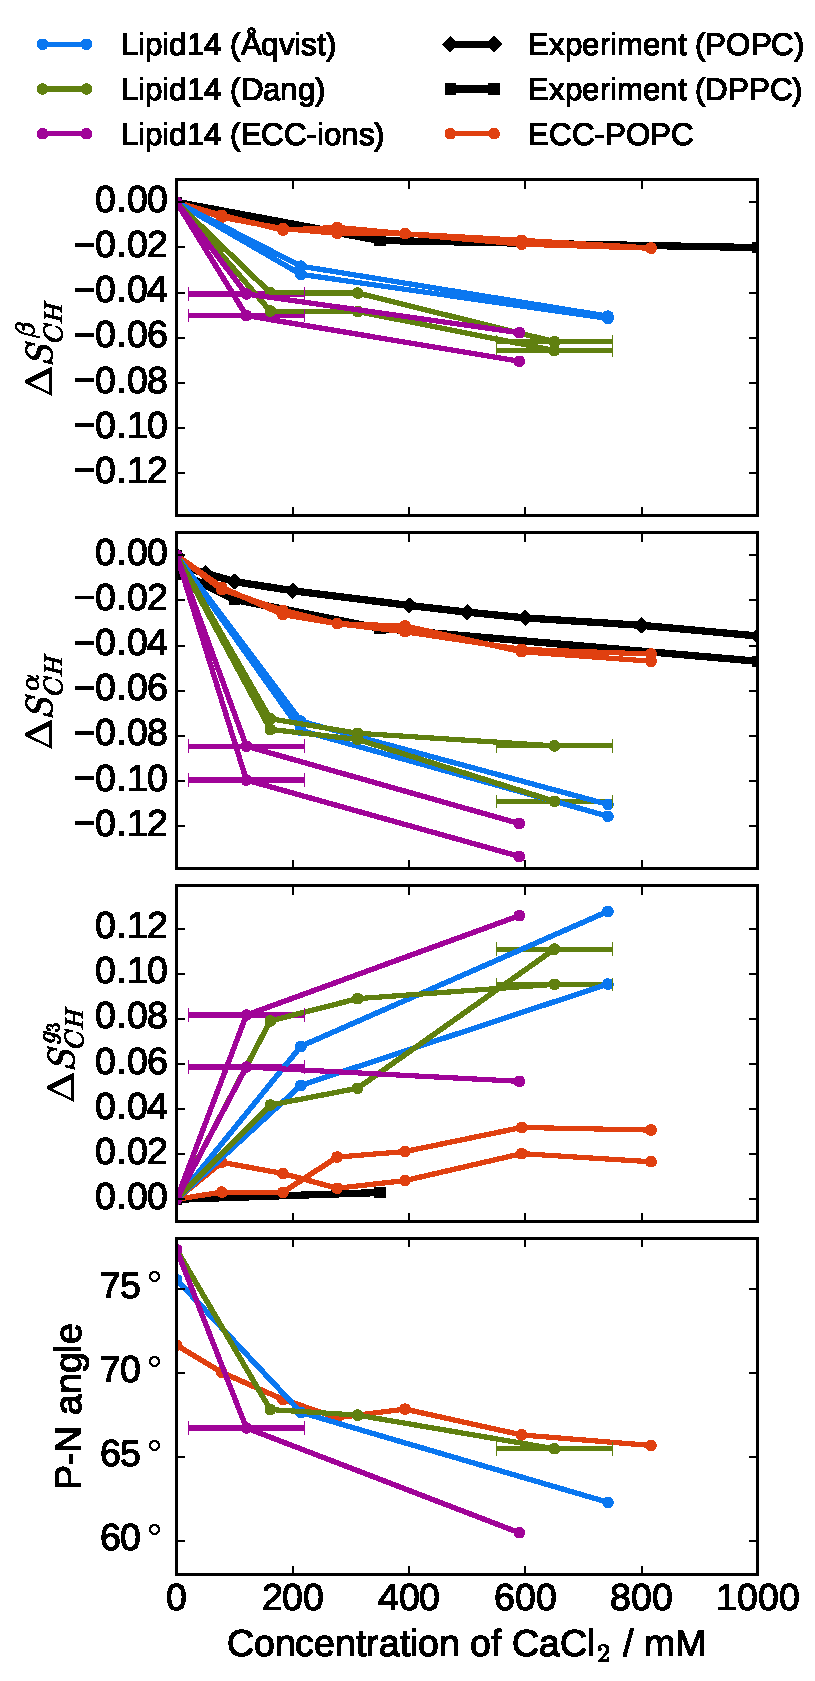
\includegraphics[width=8.0cm]{../img/ecc_popc/PN_angle_OrdPars-A-B-g3_L14-ECCL17_q80_sig89_CaCl.pdf} 
  \caption{\label{fig:delta_ordPar_CaCl} 
    Changes of the head group order parameters and P-N vector orientation of a POPC bilayer  
    as a function of the CaCl$_2$ concentration in bulk ($C_{ion}$) 
    from simulations at 313 K together with experimental data  
    (DPPC (323\,K) \citep{akutsu81} and POPC (313\,K) \citep{altenbach84}).  
    The error estimate for bulk concentrations is approximately 10\,mM. 
    The order of magnitude larger error in the
    simulation with Lipid14 and ECC-ions is due to unconverged bulk densities  (shown if Fig.~\ref{fig:cacl-dens}) limited by
    the simulation box.  
    Simulation data with Lipid14 and Åqvist ion parameters at 298 K are taken directly from 
    Refs.~\citep{lipid14POPC0mMNaClfiles,lipid14POPC350mMCaClfiles,lipid14POPC350mMCaClfilesNC}. 
  } 
\end{figure} 


Changes of the lipid bilayer head group order parameters extracted from simulations and 
experiments \citep{akutsu81, altenbach84} are shown in Fig.~\ref{fig:delta_ordPar_CaCl} 
as a function of CaCl$_2$ concentration. 
As seen in Fig.~\ref{OrderParameterCHANGESsurf}, the order parameters decrease 
proportionally to the amount of the bound positive charge. 
These results can be thus used to compare the ion binding affinities to lipid bilayers between 
simulations and experiments using the electrometer concept~\citep{seelig87, catte16}. 

The results from simulations combining the ECC-POPC with the ECC-ion models \citep{martinek17, kohagen16, Pluharova2014} exhibit a significantly improved behavior of the POPC head group order parameters as a function of NaCl or CaCl$_2$ concentrations, see Fig.~\ref{fig:delta_ordPar_NaCl} and Fig.~\ref{fig:delta_ordPar_CaCl}. Considering that we are also able to reproduce the experimental response in systems with known charge density (see above section \ref{section:boundCHARGE}), we conclude that our ECC model correctly reproduces the binding affinities of Na$^{+}$ and Ca$^{2+}$ ions to the POPC lipid bilayer. Furthermore, while the response of the glycerol backbone $g_3$ order parameter to CaCl$_2$ was significantly overestimated in the original Lipid14 model, the ECC-POPC model provides an improved agreement with experiment, as seen in Fig.~\ref{fig:delta_ordPar_CaCl}. 
Also the changes of the P-N vector angle are too pronounced for the Lipid14 model, 
for which the largest tilting toward water phase induced by a $780\,\mathrm{mM}$ 
CaCl$_2$ concentration is approximately 17$^{\circ}$. The corresponding value 
for the ECC-POPC simulation is only 6$^{\circ}$ ($820\,\mathrm{mM}$ CaCl$_2$).  

Within the Lipid14 model, the overestimated changes in the lipid headgroup order parameter of POPC  as functions of the CaCl$_2$ concentration arise both from the overestimated binding affinity and the excessive sensitivity of the headgroup tilt to the bound positive charge. It is plausible to assume that the same applies to the other lipid models tested in a previous study~\citep{catte16}, which underlines the importance of validation of the lipid headgroup order parameter response to the bound charge.  


\begin{figure}[htb!] 
  \centering 
  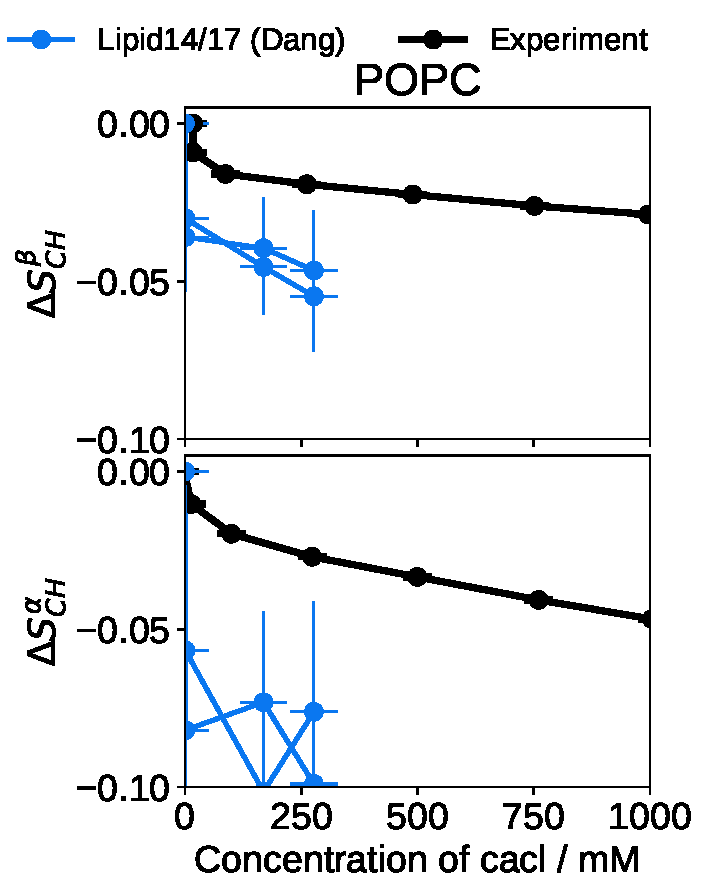
\includegraphics[width=\figwidth]{../img/ecc_pops/l17/order_parameters_changes_A-B_POPC_cacl.pdf} 
  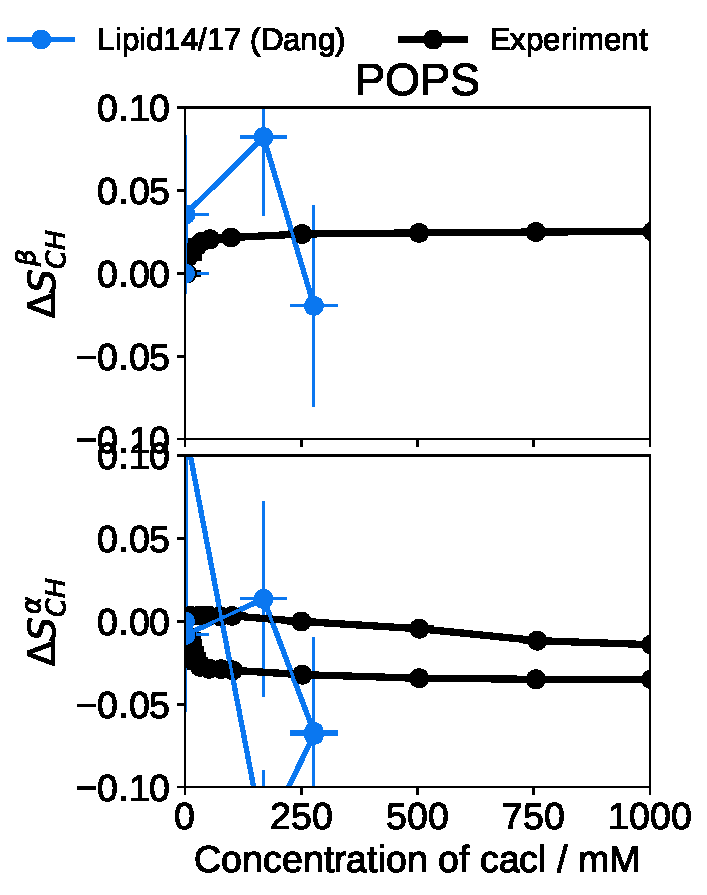
\includegraphics[width=\figwidth]{../img/ecc_pops/l17/order_parameters_changes_A-B_POPS_cacl.pdf} 
  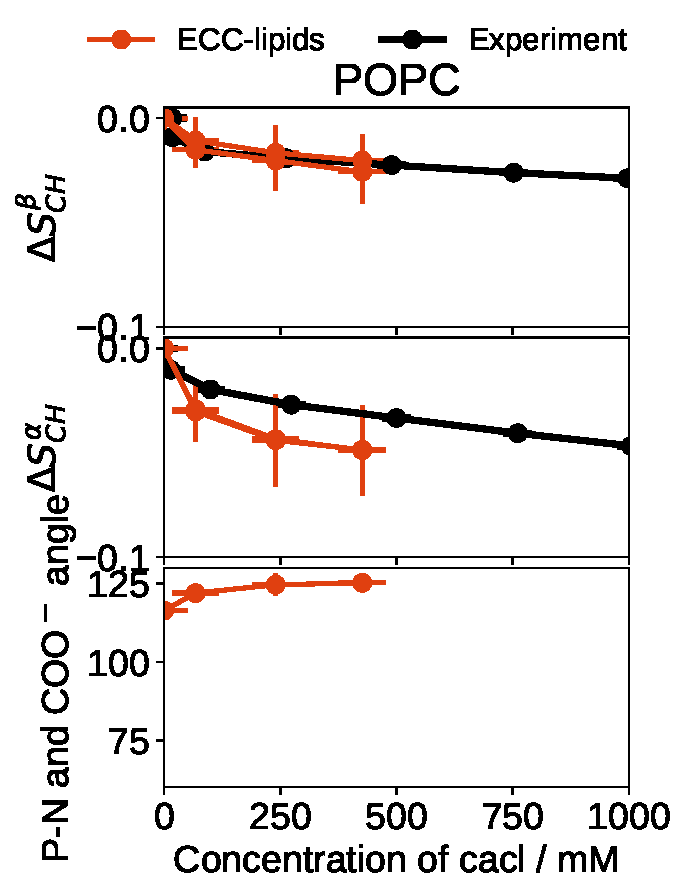
\includegraphics[width=\figwidth]{../img/ecc_pops/order_parameters_changes_A-B_POPC_cacl.pdf} 
  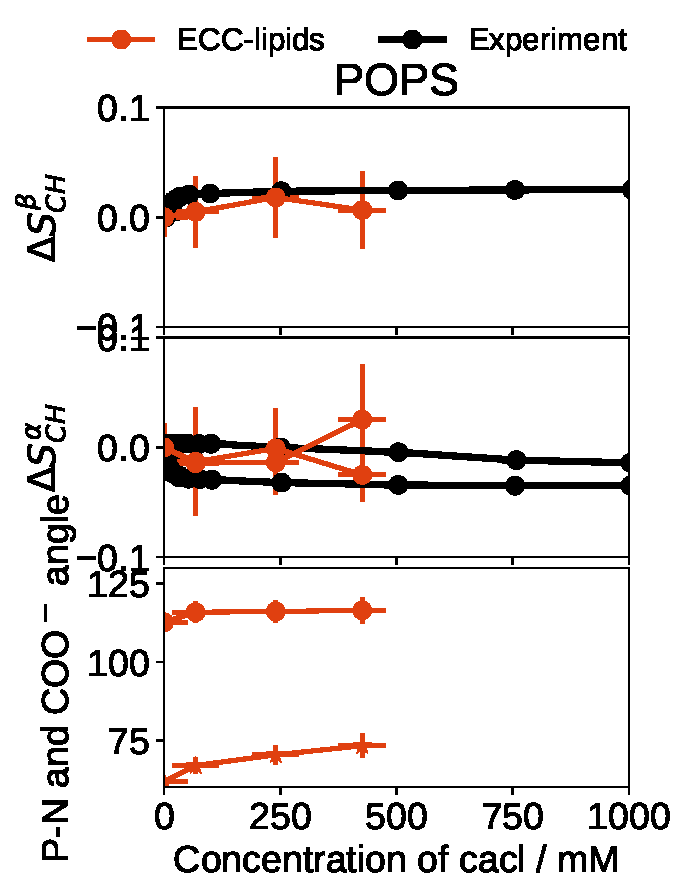
\includegraphics[width=\figwidth]{../img/ecc_pops/order_parameters_changes_A-B_POPS_cacl.pdf} 
  \caption{\label{fig:delta_ordPar_CaCl_PCPS} 
    Changes of the head group order parameters of a POPC:POPS 5:1 bilayer as a function of CaCl concentration 
    in bulk ($C_{ion}$) from simulations with different force fields at 298 K together with  
  } 
\end{figure} 


\begin{table}[tb!] 
  \caption{Bulk concentrations of Ca$^{2+}$ (C$_b$), relative surface excess of calcium with respect to water ($\Gamma_{Ca}^{\rm water}$), 
    and the percetages of Ca$^{2+}$ bound to phosphate or carbonyl oxyges ($r^\mathrm{Ca^{2+}} _\mathrm{PO_4} $ and $r^\mathrm{Ca^{2+}} _\mathrm{O_{carb.}}$) 
    in different POPC bilayer models. All systems have the same molar concentration of Ca$^{2+}$ with respect to water ($C_{ion}'$=350mM). 
  \label{tab:binding}} 
  \begin{tabular}{l|c c | c | c c} 
    model                  & $C_{ion}'$ & $C_{ion}\,/\,\mathrm{mM}$ & $\Gamma_{Ca}^{\rm water} \,/\, \mathrm{nm}^{-2}$  & $r^\mathrm{Ca^{2+}} _\mathrm{PO_4} $ & $r^\mathrm{Ca^{2+}} _\mathrm{O_{carb.}} $ \\ 
    \hline 
    ECC-POPC             &  350  &  $280\pm 10 $  &  $0.06 \pm 0.01 $                           &  99\%  &    25\%    \\ 
    Lipid14/Åqvist     &  350  &  $210\pm 10 $  &  $0.13 \pm 0.01 $                          & 100\%  &    37\%     \\ 
    Lipid14/Dang           &  350  &  $160\pm 10 $  &  $0.23 \pm 0.03 $                            & 100\%  &    14\%    \\ 
    Lipid14/ECC-ions       &  350  &  $120\pm 100$  &  $0.35 \pm 0.11 $                         & 100\%  &    23\%    \\ 
  \end{tabular} 
\end{table} 

 
 
 
Binding affinities of Ca$^{2+}$ ions to a POPC bilayer in different simulation models were quantified by calculating the relative surface excess of calcium with respect to water molecules, $\Gamma_{\rm ion}^{\rm water}$, from Eq.~\ref{surfexcess}. 
The values of $\Gamma_{\rm ion}^{\rm water}$ 
from different simulations with the same molar concetration of cations with respect 
to water ($C_{ion}'$=350mM) are shown in Table~\ref{tab:binding}. 
As expected from the changes of the lipid headgroup order parameters in Fig.~ \ref{fig:delta_ordPar_CaCl}, the relative surface excess of calcium, $\Gamma_{\rm Ca}^{\rm water}$ = 0.06~nm$^{-2}$, is significantly smaller for the ECC-POPC model than for the other models, 0.13--0.35~nm$^{-2}$. 
 
\begin{figure}[htbp!] 
  \centering 
  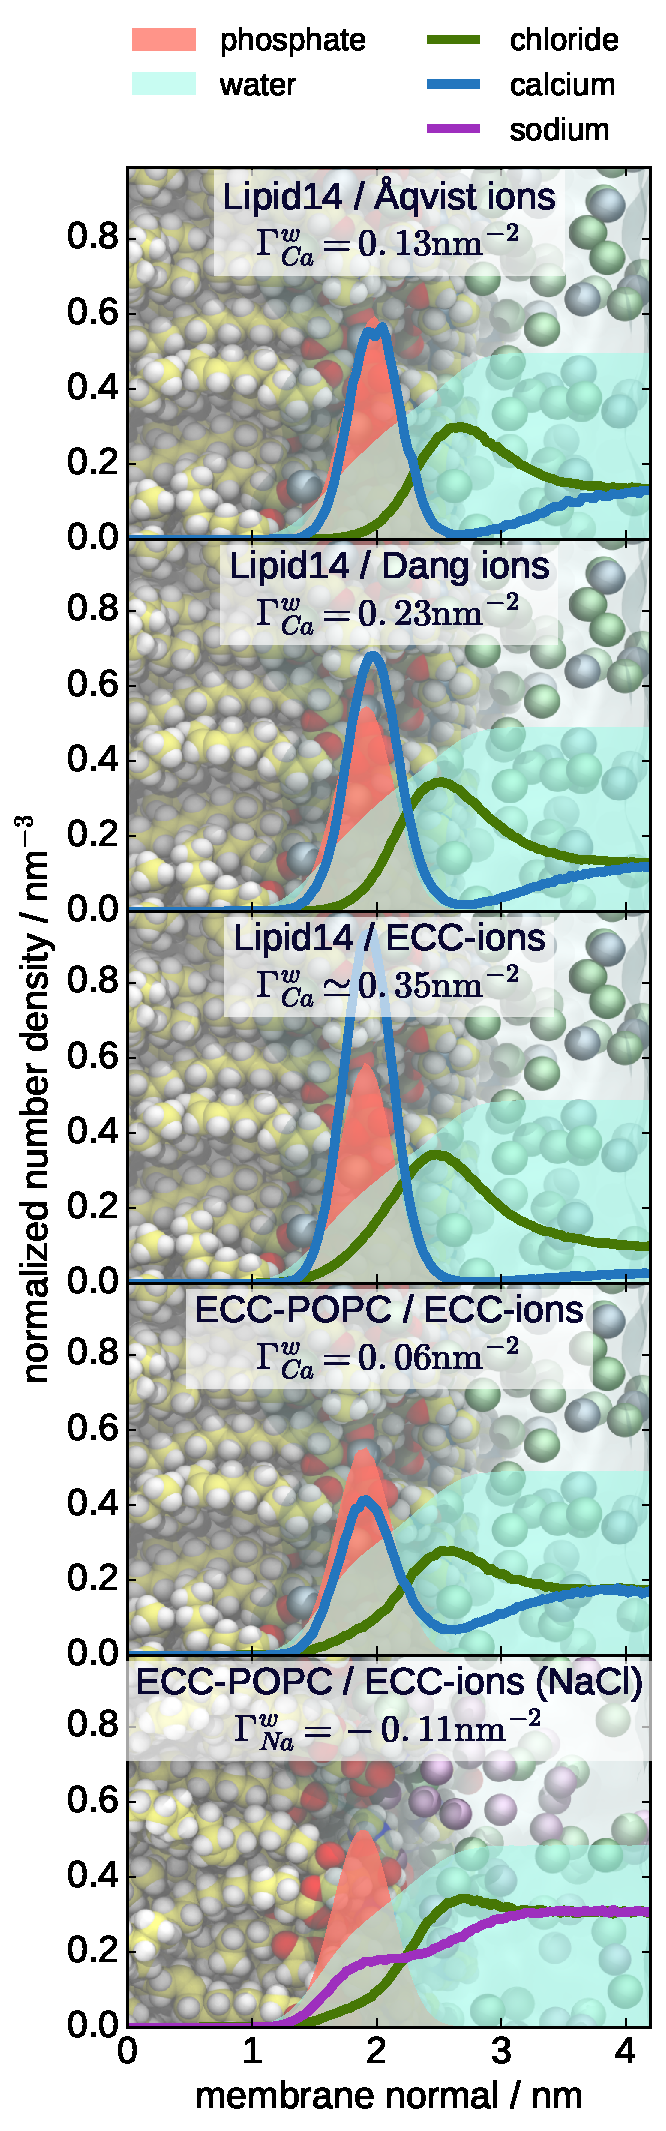
\includegraphics[height=19.9cm]{../img/ecc_popc/density_profiles_ca_cl_wat_phos_models-compar.pdf} 
  \caption{\label{fig:cacl-dens} 
    Number density profiles of \ce{Ca^{2+}}, \ce{Na^{+}} and \ce{Cl^-} along membrane normal axis 
    for different force fields. 
    In order to visualize the density profiles with a scale comparable to the profile of \ce{Ca^{2+}},  
    the density profiles of~\ce{Cl^-} and \ce{Na^{+}} ions are divided by 2, and 
    the density profiles of phosphate groups and water are divided by 5 and 200, respectively.  
    All simulations with \ce{CaCl2} shown here have the same molar concentration of ions in water ($C_{ion}'$=350~mM). 
    The simulation with \ce{NaCl} has $C_{ion}'$=1000~mM. 
    } 
\end{figure} 





\subsection{Molecular interaction and binding affinities of Ca$^{2+}$  cations to the mixed POPC:POPS (5:1) membrane} 

\todo{Provide density plots also for PC:PS mix.}

\textbf{Where do the cations bind?} 
\todo{Stationary distribution: Make a figure documenting the populations of bound \ce{Ca^{2+}} cations (like I have in the presentation) that would accompany Table \ref{tab:Ca_binding_PCPS}. 
This will roughly correspond to the PC stoichiometry plot \ref{fig:cacl_complexes}. }

The affinity towards PC and PS lipids and some of their groups was evaluated 
by counting contacts between the cation and the oxygen atoms of the lipids
similarly as was done in \cite{melcr18}. 
The threshold for counting a contact was set to be $0.3 \mathrm{nm}$, 
which encompasses the first peak of radial distribution function between the cations and the oxygen atoms of the lipids. 
\todo{Show a figure of RDF documenting this?}

The percentages of the populations of membrane-bound calcium cations for various membrane moieties 
are summarized in Table~\ref{tab:Ca_binding_PCPS}.
Although the lipid ratio in the membrane is 5~PC:1~PS,
approximately half of the total population of bound calcium cations is in contact with PS lipids
with 7\% bound only to them. 
This corroborates the intrinsincally higher affinity of PS lipids to calcium cations compared to PC lipids. 

Cations that are bound only to PC in the mixed bilayer with PS 
behave similarly as in the pure PC bilayer
maintaining similar probabilities for clustering one, two or even three PC lipids together. 

The population analysis also suggests 
that the calcium cations prefer to reside in the phosphate region of the membrane. 
Such a finding is further validated with a more detailed analysis using Markov state modeling (MSM) \citep{Pande_MSM_paper} \todoi{Add papers reviewing MSM, e.g. recent Pande's paper.}. 
The set of states of a calcium cation 
encompassed all possible combinations of up to three surrounding lipids. 
In the case of PC, we used only the phosphate moitety, which forms the dominant contribution for calcium binding.
For PS we also distinguished configurations in which calcium interacts with the carboxylate moiety. 
All possible combinations of such states were used to build a Markov model at a lag time $25\,\mathrm{ns}$ using pyEMMA code by \citet{pyemma} \todoi{add citation for pyemma}. 
The resulting MSM was validated using Chapman-Kolmogorov test \citep{FrankNoe_papers_MSM} \todoi{Add citation for Noe's papers on MSM, especially Chapman Kolmogorov test.}. 
The stationary distribution of the states reveals a strong preference of the calcium cations to reside in the phosphate region of the mixed PC-PS membrane. 
When interacting with PS, configurations with the phosphate moiety from either PC or PS dominate the population.
Moreover, states containing interactions with the carboxylate group in PS 
bear higher probability when interacting also with the phosphate group of the same lipid or other lipids. 
The interactions of the carboxylate group in PS with calcium and other phosphate groups
sheds light into the qualitatively different response of the head group order parameters $\alpha$ and $\beta$ in PS compared to PC 
(see Figs.~\ref{fig:delta_ordPar_CaCl} and~\ref{fig:delta_ordPar_CaCl_PCPS}). 
\todo{Add figures showing the shift of the distribution of a COO- orientation w/o \ce{CaCl2}.}



The increased response of head group order parameters $\alpha$ and $\beta$ of PC, which form the lipid electrometer concept,
in mixed 5~PC:1~PS bilayer compared to pure PC
is due to higer affinity of the membrane mediated by even a relatively small fraction (1/6) of PS lipids. 
This is in line with the steep onset of the response of the PS head group order parameters at lower concentrations.
The complex response of the head group order parameters of PS lipids 
is due to the confomational change of the carboxylate group that is attracted more towards the phosphate region. 



\begin{figure}[tb]
  \centering
  \includegraphics[width=8.0cm]{../img/ecc_popc/histogram_bound_times_ECC-lipids_346mM_CaCl.pdf} 
  \includegraphics[width=8.0cm]{../img/ecc_pops/histogram_bound_times_ECC-lipids_346mM_CaCl.pdf}
  \caption{\label{fig:hist_residence_times}
   Histograms of residence times of \ce{Ca^{2+}} in a POPC bilayer
   from ECC-POPC (top) and CHARMM36 (bottom) simulations with ECC-ions.
   Both simulations had the same concentration of \ce{CaCl_2} respect to water ($C_{ion}'$= 450~mM).
   CHARMM36 simulation was directly taken from Refs.~\citenum{javanainen17,zenodo.259376}.
   Scales of x-axes represent the lengths of the simulations used for analysis.
   In ECC-POPC simulation, 90\% of the residence times are
   shorter than $60\,\mathrm{ns}$, % exactly $53\,\mathrm{ns}$                                                                          
   with the longest observed residence time being $141\,\mathrm{ns}$,
   which is well below the total length of the simulation (200~ns).
   This is, however not the case in CHARMM36 simulation,
   where residence times of several calcium cations are    
   apparently limited by the length of the simulation.
   %With such a simulation, which is relatively short for the employed model,
   %we can merely estimate an upper bound that
   %only
   Less than 60\% of the residence times are
   %is formed by cations interacting with the phospholipid membrane
   shorter than the half of the simulation length~(400~ns)
   in CHARMM36 simulation.
  }
  \todo{Put the figures into the repository and modify the caption. }
\end{figure}


\todo{Timescales: Comment implied timescales and the MFPT (mean first passage times) and the associated states that contribute to the slowest transitions. 
Get MFPT also for pure PC. 
Give upper limit of residence time for 90\% of population (as in ECC-POPC paper) -- it is $142$~ns, longest observed $521$~ns.}
Timescales associated with the binding of calcium cation from solution to the membrane
are plotted for each binding event as a histogram in Fig.~\ref{fig:hist_residence_times}. 
Using these plots, we can estimate the upper bound for the residence time of a calcium cation 
to be lower than $60\,\mathrm{ns}$ for pure POPC neutral bilayer 
and shorter than $150\,\mathrm{ns}$ for the mixed 5\,PC:1\,PS negatively charged bilayer. 
The longest observed residence times in the simulations were $141\,\mathrm{ns}$ for the neutral membrane 
and $521\,\mathrm{ns}$ for the negatively charged membrane. 
In addition to such estimates of the time scales, we used the Markov model on top of the simulation with the negatviely charged mixed bilayer
to calculate the time of the mean first passage of calcium from solution to the membrane (and in reverse) resulting in $55\,\mathrm{ns}$  ($165\,\mathrm{ns}$). 

\todo{Fluxes: committor analysis, dominant fluxes (table and figure)}
From the spectrum of the transition matrix, we also observe that 
the slowest transitions are associated with the binding to two or three phosphate moieties from either PC or PS,
which are also among the states with the highest probabilities.
The net fluxes of calcium cations from solution to such states also form a large contribution to the total flux ($\approx 45\%$). 
\todo{Make a table and a figure of the state probabilities and fluxes to support this statement.}. 
Analysis of the possible binding pathways of calcium cations to the negatively charged mixed bilayer 
reveal that the cations mostly enter the membrane bound states directly from solution 
without complicated transitions at the time scales of the order of the lag time of the Markov state model, $25\,\mathrm{ns}$. 










 
\begin{table}[tb!] 
\begin{centering}
  \caption{Bulk concentrations of Ca$^{2+}$ (C$_b$), 
           and the percentages of the population 
           of bound Ca$^{2+}$ to either to PC or PS, 
           to PC or PS without PS--phosphate group,
           to PC or PS without PS--carboxylate group,
           to PC and PS simultaneously,
           only to PC, 
           and only to PS 
           in a mixed POPC:POPS (5:1) bilayer. 
          \label{tab:Ca_binding_PCPS} } 
          \todo{transpose this table and remove the comparison with Lipid14/17}
  \begin{tabular}{ l | r } 
	model   & ECC-lipids  \\
	\hline
	$C_{ion}\,/\,\mathrm{mM}$  &  $240\pm 10 $  \\
	\hline
	PC+PS  &  100  \\
	PC+PS no PO$_4$  &  98-99  \\
	PC+PS no COO$^-$ &  100  \\
	PC-$Ca^{2+}$-PS  &   43  \\
	PC only          &   50  \\
	PS only          &    7  \\ 
	\hline 
  \end{tabular} 
\end{centering}
\end{table} 



 
\subsection{Molecular interactions between Ca$^{2+}$ cations and POPC oxygens} 
We analyzed the ratio of the number of calcium cations bound to either phosphate or carbonyl moieties and the total number of bound cations in our POPC bilayers as done previously in Ref.~\citep{javanainen17}. A maximum distance of 0.3~nm from any lipid oxygen is used to define a bound calcium. The results from ECC-POPC simulation in Table~\ref{tab:binding} show that almost all (99\%) of the bound Ca$^{2+}$ ions are in direct contact with phosphate oxygens. From these ions, only one third (32\%) also interacts with the carbonyl oxygens, while the interaction of calcium ions with carbonyl oxygens only is rare (1\%). The most abundand interaction scenarios between Ca$^{2+}$ ions and phosphate oxygens are visualized using the probability density isocontours in Fig.~\ref{fig:volmaps}. While higher concentrations of \ce{CaCl2} increase the number of contacts per lipid, the distribution of contacts between phosphate and carbonyl oxygens is not affected. 
 
\todo{Analyze the orientation of the carbonyls and plot it as a violin plot/probability density. Change the following discussion afterwards.}
In the case of POPC, the $C_2$ segment in {\it sn}-2 chain shows a low order parameter with a small forking as measured in experiments by \citet{seelig75,schindler75,gawrisch92}. 
This feature has been suggested to indicate that the carbonyl
of {\it sn}-2 chain is directed towards the water phase, in contrast to the
carbonyl in {\it sn}-1 chain, which would orient more along the bilayer
plane~\cite{seelig75,schindler75,gawrisch92}. This may be an important
feature for the ion binding details, which it is not fully reproduced by other
available lipid models~\cite{ollila16}.

\begin{figure}[tb!] 
  \centering 
  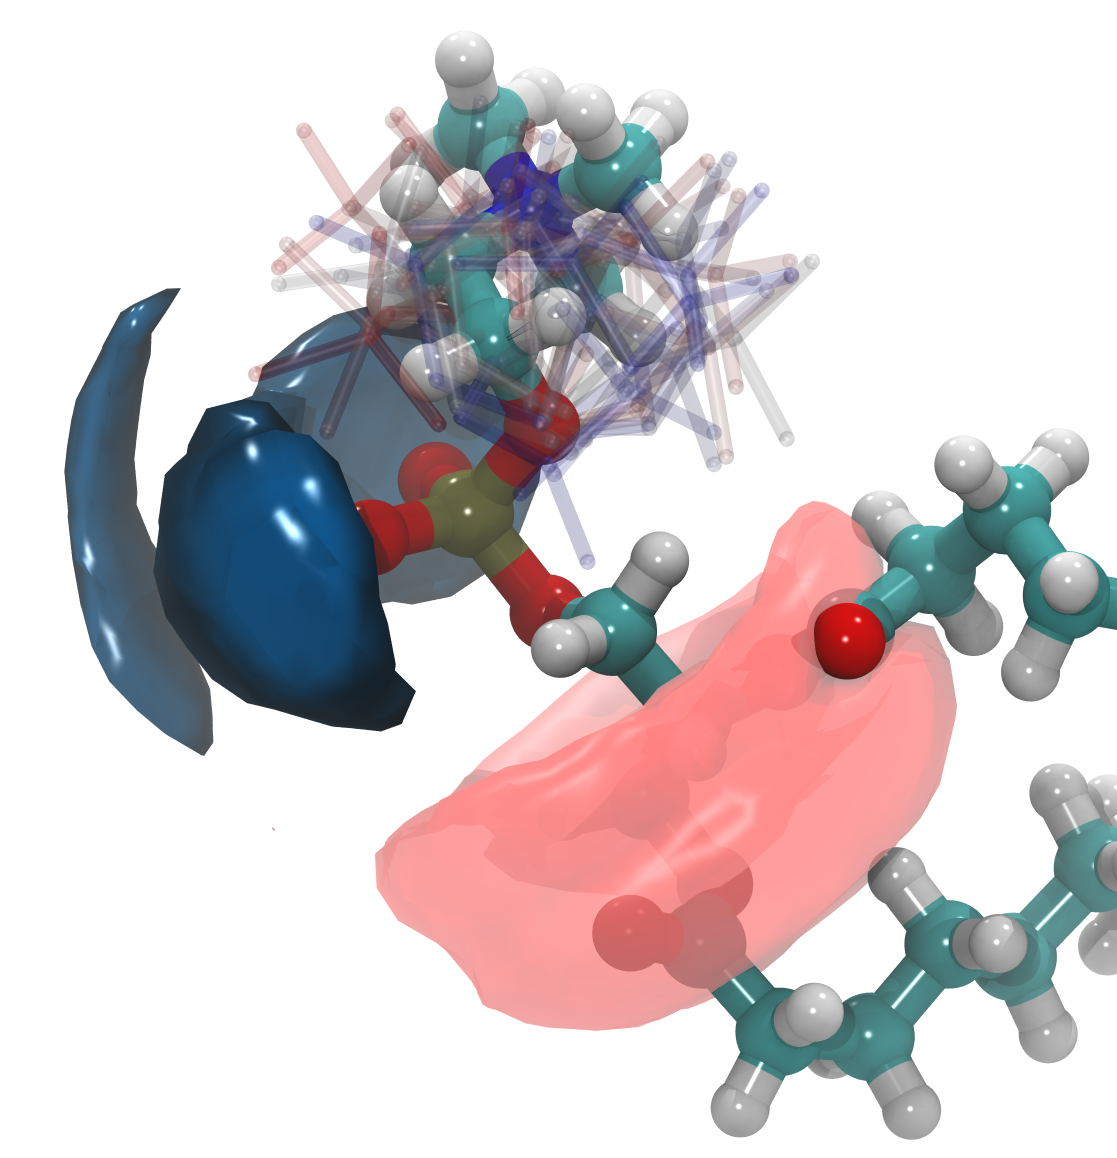
\includegraphics[width=8.0cm]{../img/ecc_popc/isocontours_r37_ca_O-carb.png} 
  \caption{\label{fig:volmaps} 
    Isocontours of spatial number density of \ce{Ca^{2+}} (dark blue, 0.001~Å$^{-3}$) 
    and POPC carbonyl oxygen atoms (light semi-transparent red, 0.008~Å$^{-3}$, all POPC lipids contribute). 
    Calcium cations localize mostly around phosphate oxygens (oxygens red, phosphorus bronze).
    Interactions with carbonyl oxygens is less likely than with phosphate oxygens, 
    and it is contributed more by other neighbouring phospholipids than by the same lipid. 
    Transparent structures are shown to depict the variability of choline configurations 
    (colour warps from red to blue along the simulation time). 
    The number density was evaluated for each lipid, 
    after its structural alignment using only phosphate group.
    MDAnalysis \citep{mdanalysis2011} library was used for 
    the calculations of the structural alignment and the spatial number density. 
    VMD \citep{hump96} was used for visualisation. 
    Carbon atoms are depicted in cyan, hydrogen atoms in white, oxygen atoms in red, nitrogen in blue.
  } 
\end{figure} 
 
 
In conclusion, the results suggest that calcium ions bind specifically to the phosphate oxygens, occasionally interacting also with the carbonyls of the PC lipids. This is in a qualitative agreement with previous conclusions from several experimental studies~\citep{hauser76, hauser78, herbette84, cevc90, binder02}. However, the present results suggest, in 
agreement with experiments, an overally weaker binding to the bilayer, in particular with a lower relative binding affinity to the carbonyls than inferred from previous MD simulation studies~\citep{bockmann03, bockmann04, melcrova16, javanainen17}. 

 
\subsection{Binding stoichiometry of \ce{Ca^{2+}} cations to POPC membrane} 
Simple binding models have been used previously to interpret the same experimental data \citep{altenbach84,macdonald87} as employed in this work to validate the simulation models (Fig.~\ref{fig:delta_ordPar_CaCl}). In particular, NMR data concerning the PC headgroup order parameters response and atomic absorption spectra were explained best using a ternary complex binding model with a binding stoichiometry of one \ce{Ca^{2+}} per two POPC lipids~\citep{altenbach84}. Nevertheless, a Langmuir adsorption model assuming a \ce{Ca^{2+}}:POPC stoichiometry of 1:1 also provided a good fit to the experimental data when considering \ce{CaCl2} at low concentrations only~\citep{macdonald87}. 
 
 
In this work, we reproduce the same experimental data used to infer binding stoichiometries employing our ECC-POPC model. Thanks to our simulations, we have a direct access to atomistic details of the binding stoichiometry without a need for any binding model as employed for interpreting in experiments~\citep{altenbach84, macdonald87}.
To evaluate the relative propensities for each of the stoichiometric complexes (i.e.,~1~Ca$^{2+}$:~n~POPC),
we calculated for each bound Ca$^{2+}$ the number of POPC molecules having oxygen atoms within a distance of 0.3~nm.
Results from the POPC bilayer simulation with a 285~mM bulk concentration of CaCl$_2$ are shown in Fig.~\ref{fig:cacl_complexes}. 
We found the largest propensity for the 1:2 complex (41\%), with probabilities of complexes with the stoichiometries of 1:1~(25\%)~and 1:3~(34\%)~being only slightly lower. This suggests a more complex binding model than considered in a simple 1:2 ternary complex model previously. Nevertheless, with a broad brushstroke, the simulation data can be viewed such that one calcium binds to two lipids on average, because the probabilities of the complexes with 1 or 3 lipids are almost equal to each other  (and complexes with more than three lipids per one calcium ion were not observed). This probably explains why the simple the ternary complex model fits adequately the experimental data, as well as the ECC-POPC simulation results (see Fig.~S3 in SI). 
 
\begin{figure}[tb!] 
  \centering 
  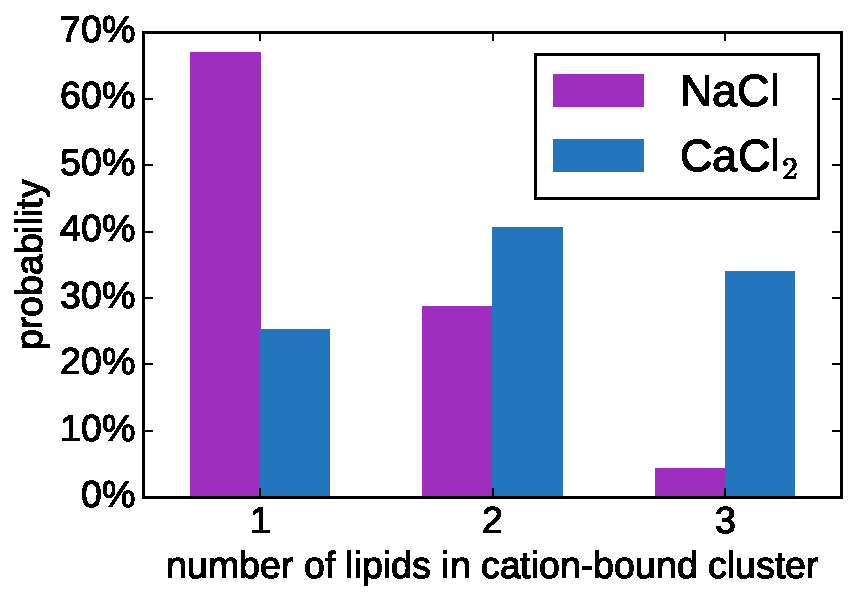
\includegraphics[width=8.0cm]{../img/ecc_popc/stoichiometry_NaCl-CaCl2_comparison_Ecc-lipids.pdf} \\ 
  \caption{\label{fig:cacl_complexes} 
      Relative probabilities of existence of \ce{Na^{+}} or \ce{Ca^{2+}} complexes 
      with a certain number of POPC lipids.  
      \ce{Na^{+}} complexes were evaluated from the simulation with 1~M concentration; 
      and \ce{Ca^{2+}} complexes were evaluated from the simulation with 287~mM concentration. 
  } 
\end{figure} 
 
 
 
 
\subsection{Residence times of \ce{Ca^{2+}} cations in the POPC membrane} 
 
Equilibration of \ce{Ca^{2+}} ions at a POPC bilayer in MD simulations is a microsecond time scale process with current force fields, such  as CHARMM36 and Slipids force fields~\citep{javanainen17}. This suggests that at least several microseconds are required to reach the ion binding/unbinding equilibrium. 
To quantify the exchange of ions between the membrane and aqueous solution in simulations, we evaluated residence times of ions bound to the membrane. Within our analysis, an ion is considered to be bound when it is within 0.3~nm from any oxygen atom belonging to a POPC molecule. 
 
The histograms of residence times of \ce{Ca^{2+}} in a POPC bilayer ($C_{ion}'$ = 450~mM) from simulations with  
ECC-POPC and CHARMM36 (simulation from Refs.~\citep{javanainen17,zenodo.259376}) are shown in Fig.~S4 in SI. 
In the CHARMM36 simulation, a significant number of the calcium ions is bound to the membrane for the whole length of the trajectory (800~ns). 
In contrast, at least an order of magnitude faster bound/unbound calcium exchange is observed within the ECC-POPC model, 
where 90\% of the \ce{Ca^{2+}} residence times to a POPC membrane are shorter than $60\,\mathrm{ns}$. The longest observed 
residence time is around 150~ns, which is below the total length of the simulation used for analysis, i.e., 200~ns. 
Note that these results are in line with the experimental estimate that the residence time of \ce{Ca^{2+}} at each PC 
headgroup is of the order of $10\,\mu\mathrm{s}$~\citep{altenbach84}. 
 
In summary, the results from the ECC-POPC model suggest that the exchange of calcium between the POPC bilayer and the solvent occurs within the $\sim$100~ns timeframe, which is significantly faster than observed in simulations emloying most of the presently available lipid models~\citep{javanainen17}. Sodium cations exhibit an even more rapid exchange between the membrane and the aqueous solution. Our results suggest that simulations with a length of several hundreds of nanoseconds are sufficient to simulate alkali and alkali earth ion binding to phospholipid bilayers in equilibrium when realistic force fields are used. This has not been the case with previous lipid force fields, which overestimate the binding strength of the sodium and, in particular,  calcium cations \citep{javanainen17, catte16}. 
 
 








\section{Interactions of neutral and negatively charged phospholipid membranes with K$^+$, Na$^+$}

\todo{Rewrite this whole section.}

\begin{figure}[htb!] 
  \centering 
  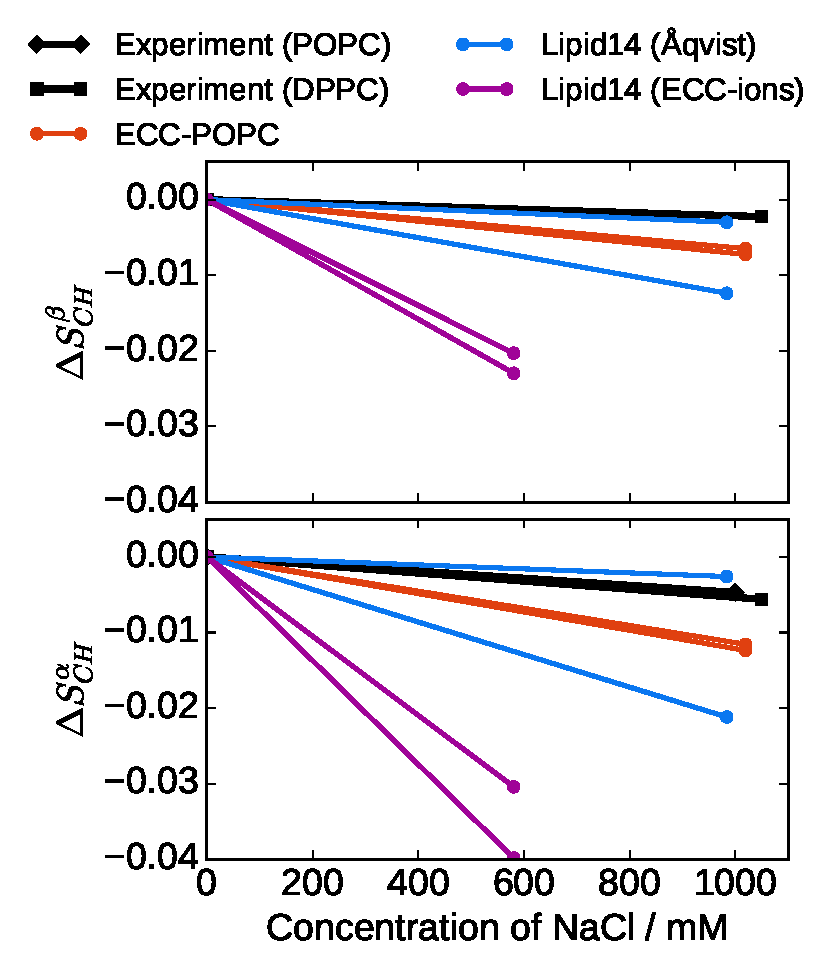
\includegraphics[width=8.0cm]{../img/ecc_popc/OrdPars-A-B_L14-ECCL17_q80_sig89_NaCl.pdf} 
  \caption{\label{fig:delta_ordPar_NaCl} 
    Changes of the head group order parameters of a POPC bilayer as a function of NaCl concentration 
    in bulk ($C_{ion}$) from simulations with different force fields at 313 K together with  
    experimental data for DPPC (323\,K) \citep{akutsu81} and POPC (313\,K) \citep{altenbach84}. 
    Simulation data with Lipid14 and Åqvist ion parameters at 298 K are taken directly from 
    Refs.~\citep{lipid14POPC0mMNaClfiles,lipid14POPC1000mMNaClfiles}. 
  } 
\end{figure} 
 
 
Changes of the lipid bilayer head group order parameters extracted from simulations and 
experiments \citep{akutsu81, altenbach84} are shown in Figs.~\ref{fig:delta_ordPar_NaCl} 
and~\ref{fig:delta_ordPar_CaCl} as functions of NaCl or CaCl$_2$ concentrations. 
As seen in Fig.~\ref{OrderParameterCHANGESsurf}, the order parameters decrease 
proportionally to the amount of the bound positive charge. 
These results can be thus used to compare the ion binding affinities to lipid bilayers between 
simulations and experiments using the electrometer concept~\citep{seelig87, catte16}. 
 
The experimentally measured small order parameter 
changes with NaCl (Fig.~\ref{fig:delta_ordPar_NaCl})  
are reproduced by the Lipid14 model simulated with Åqvist ions. 
However, the same combination of models overestimates the order parameter changes with CaCl$_2$ (Fig.~\ref{fig:delta_ordPar_CaCl}). 
Replacing Åqvist ions with ion parameters by Dang et al.~\citep{smith94, chang1999, dang2006} 
or ECC-ions~\citep{martinek17, kohagen16, Pluharova2014} did not improve 
the results~(Figs.~\ref{fig:delta_ordPar_NaCl} and \ref{fig:delta_ordPar_CaCl}). 
In line with the previous work \citep{catte16}, the results suggest that improvements 
in the lipid parameters are required to correctly describe the binding of cations to phospholipid bilayers. 
 
\todo{convert this paragraph into a NaCl-only. }
The results from simulations combining the ECC-POPC with the ECC-ion models \citep{martinek17, kohagen16, Pluharova2014} exhibit a significantly improved behavior of the POPC head group order parameters as a function of NaCl or CaCl$_2$ concentrations, see Fig.~\ref{fig:delta_ordPar_NaCl} and Fig.~\ref{fig:delta_ordPar_CaCl}. Considering that we are also able to reproduce the experimental response in systems with known charge density (see above section \ref{section:boundCHARGE}), we conclude that our ECC model correctly reproduces the binding affinities of Na$^{+}$ and Ca$^{2+}$ ions to the POPC lipid bilayer. Furthermore, while the response of the glycerol backbone $g_3$ order parameter to CaCl$_2$ was significantly overestimated in the original Lipid14 model, the ECC-POPC model provides an improved agreement with experiment, as seen in Fig.~\ref{fig:delta_ordPar_CaCl}. 
Also the changes of the P-N vector angle are too pronounced for the Lipid14 model, 
for which the largest tilting toward water phase induced by a $780\,\mathrm{mM}$ 
CaCl$_2$ concentration is approximately 17$^{\circ}$. The corresponding value 
for the ECC-POPC simulation is only 6$^{\circ}$ ($820\,\mathrm{mM}$ CaCl$_2$).  

% on the binding affinity using surface excess:
Interestingly, the calculated relative surface excess of \ce{NaCl} at $1\,\mathrm{M}$ concentration (ECC-ions~\citep{Pluharova2014}) using our ECC-POPC model is not only quantitatively but also qualitatively different from \ce{CaCl2} having actually a negative value of $\Gamma_{Na}^{water} = -0.11 \pm 0.01) \rm{nm}^{-2}$ (Fig.~\ref{fig:cacl-dens}. This  
means that on average water molecules are preferred to sodium and chloride ions at the membrane-water interface.   
This is in contradiction with most of the available lipid force fields, which predict a positive surface excess of sodium at PC lipid bilayers \citep{catte16}. 
 
Even though \ce{Na+} ions do not bind strongly to a POPC bilayer, they still interact mostly with its oxygen moieties. 
The results from a simulation at a $1\,$M \ce{NaCl} concentration show that 55\% of \ce{Na+} ions at the bilayer interact with phosphate oxygens of POPC only and 20\% with carbonyl oxygens only, with the remaining 25\%, is interacting with both negatively charged groups. 
Sodium ions, which do not exhibit any appreciable affinity for the bilayer, also interact primarily with phosphate oxygens of the POPC, but in contrast to calcium, the interactions purely with carbonyls are also significant. 
 
The probabilities of different complexes formed by \ce{Na+} ions and POPC 
analyzed from the simulation with the ECC-POPC model at $1\,$M concentration of NaCl are also  
shown in Fig.~\ref{fig:cacl_complexes}. In contrast to calcium, the 
probability is largest (67\%) for 1:1 complex, significantly smaller (29\%) 
for 1:2 complexes and very small (4\%) for 1:3 of \ce{Na+}:POPC complexes. 
 
Note that the exchange of \ce{Na+} ions at the POPC membrane 
is yet another order of magnitude faster, with 90\% of the residence times smaller than~1~ns and the longest residence time being~6~ns. 
 
Finally, the ion binding affinities for the ECC-POPC model with different water models are compared in SI. In general, the performance of ECC-POPC with any of the tested water models is better than that of the original Lipid14 model, with the order parameter changes being slightly overestimated with the four-site water models and with TIP3P model. 
 

\todo{The PC:PS figures will be eventually combined.}


% ============================== 
% ==  ECC-lipids plots ========= 
% ==     and           ========= 
% ==  Lipid14/17 plots ========= 
% ============================== 
\begin{figure}[htb!] 
  \centering 
  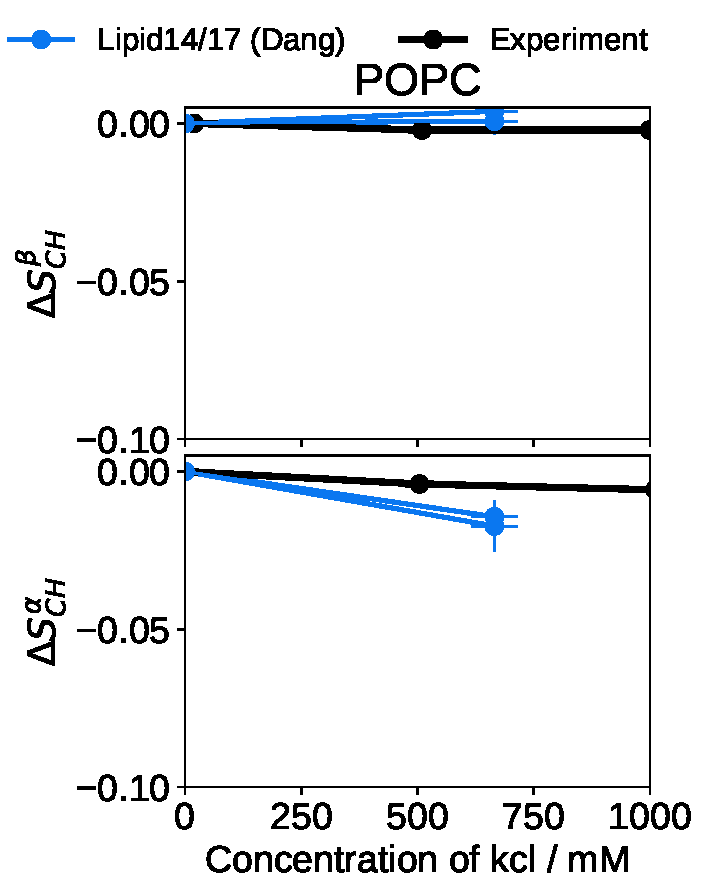
\includegraphics[width=\figwidth]{../img/ecc_pops/l17/order_parameters_changes_A-B_POPC_kcl.pdf} 
  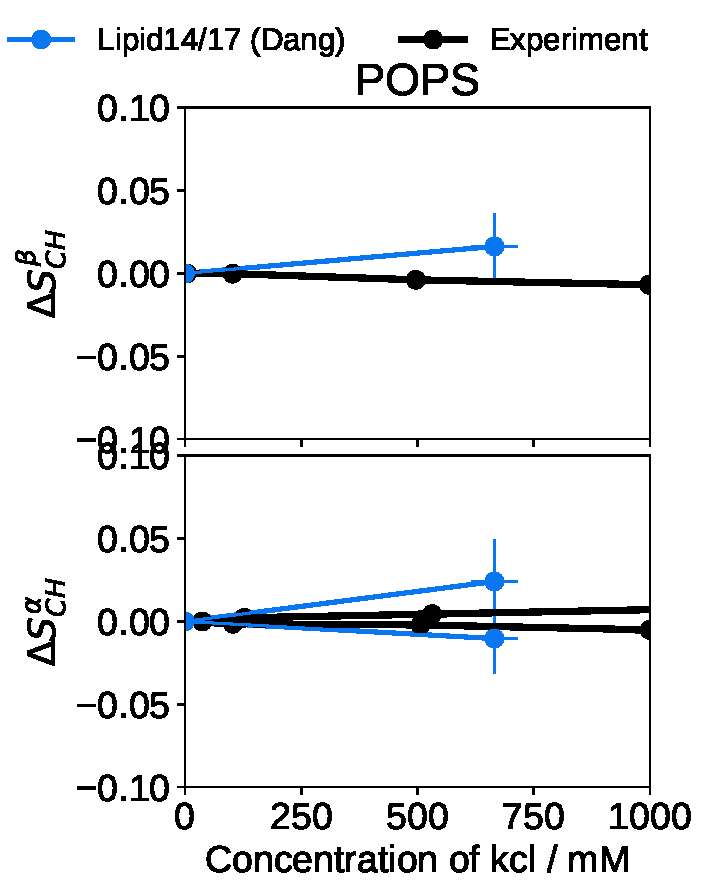
\includegraphics[width=\figwidth]{../img/ecc_pops/l17/order_parameters_changes_A-B_POPS_kcl.pdf} 
  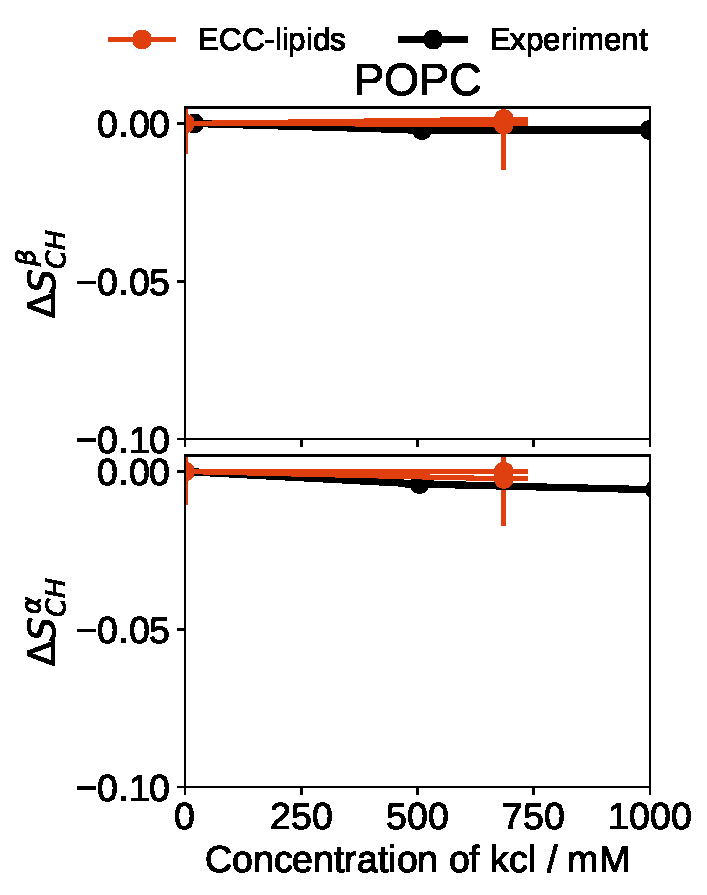
\includegraphics[width=\figwidth]{../img/ecc_pops/order_parameters_changes_A-B_POPC_kcl.pdf} 
  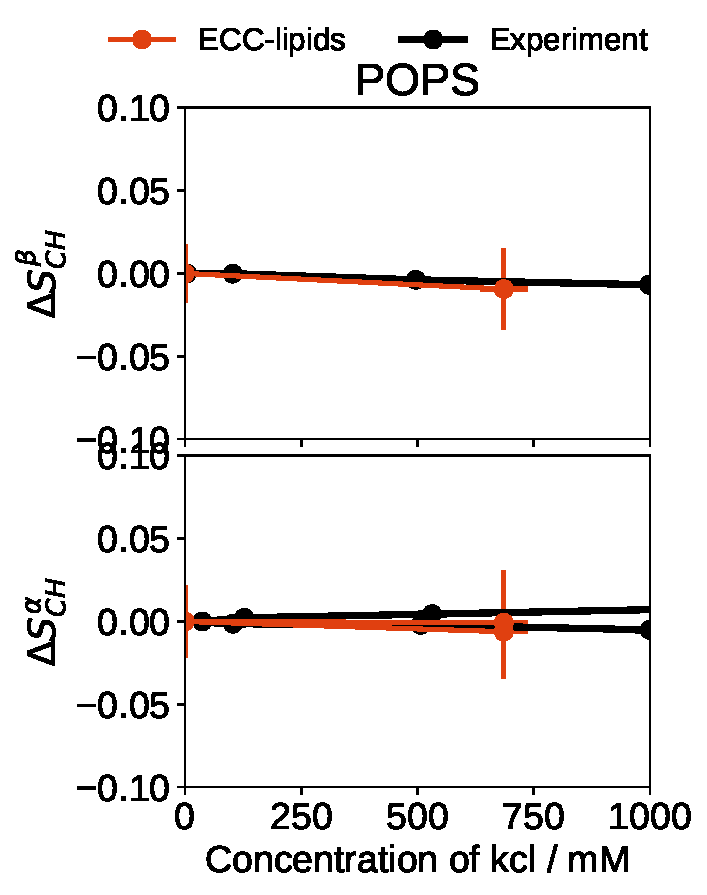
\includegraphics[width=\figwidth]{../img/ecc_pops/order_parameters_changes_A-B_POPS_kcl.pdf} 
  \caption{\label{fig:delta_ordPar_KCl} 
    Changes of the head group order parameters of a POPC:POPS 5:1 bilayer as a function of KCl concentration 
    in bulk ($C_{ion}$) from simulations with different force fields at 298 K together with  
  } 
\end{figure} 
 
 
\begin{figure}[htb!] 
  \centering 
  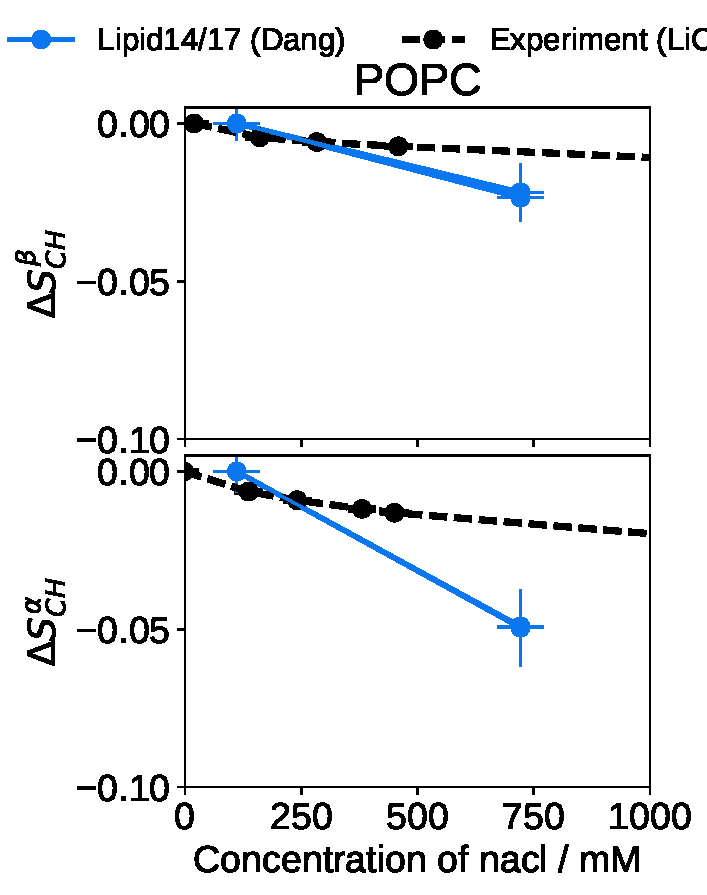
\includegraphics[width=\figwidth]{../img/ecc_pops/l17/order_parameters_changes_A-B_POPC_nacl.pdf} 
  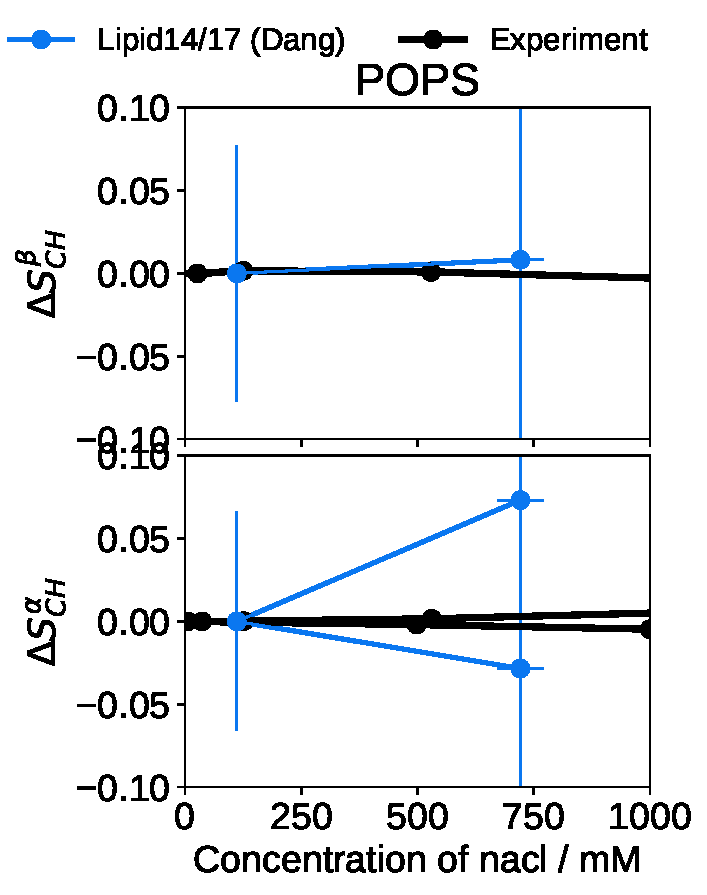
\includegraphics[width=\figwidth]{../img/ecc_pops/l17/order_parameters_changes_A-B_POPS_nacl.pdf} 
  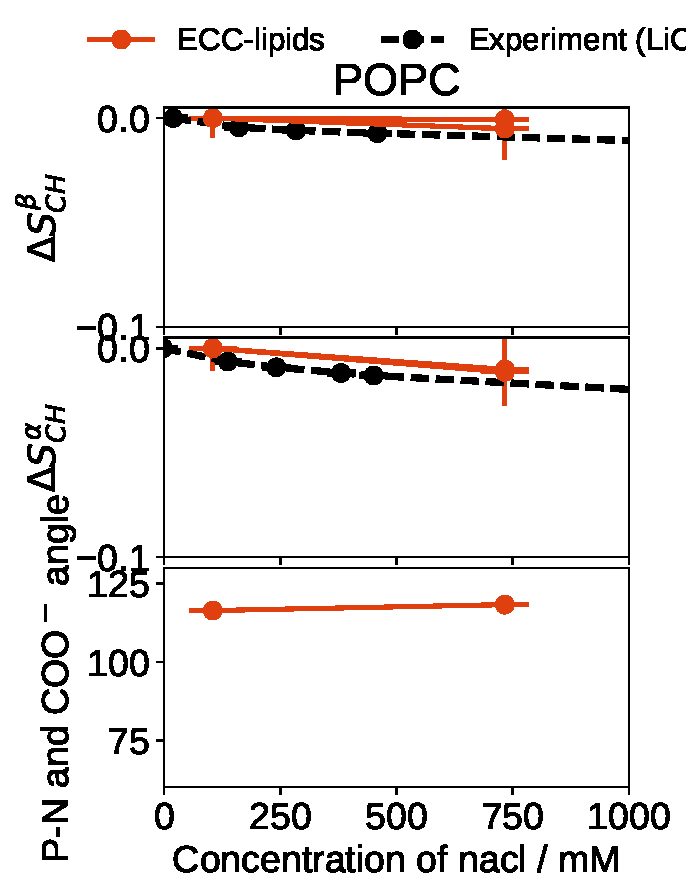
\includegraphics[width=\figwidth]{../img/ecc_pops/order_parameters_changes_A-B_POPC_nacl.pdf} 
  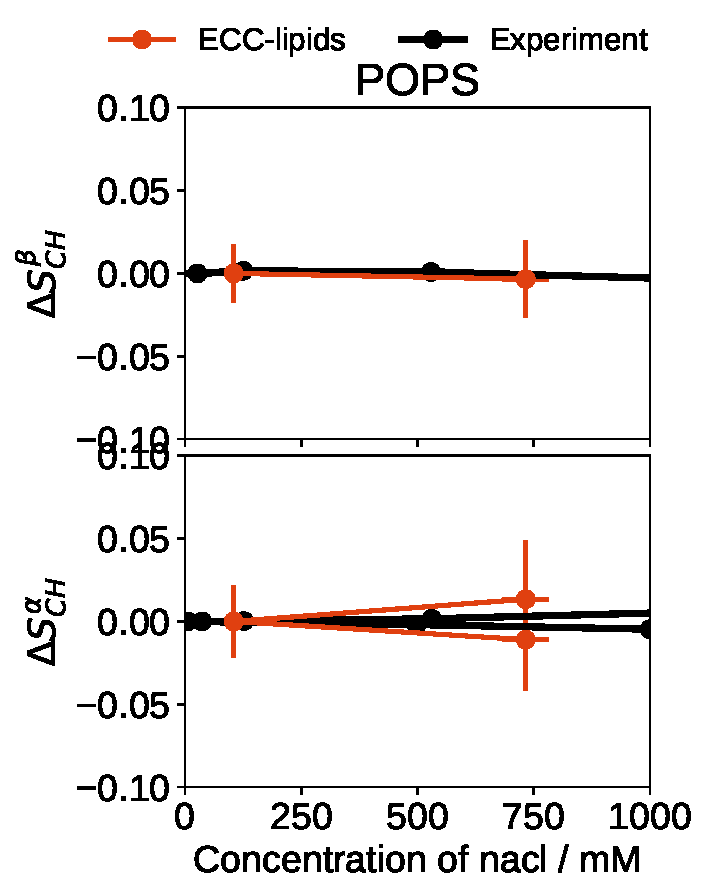
\includegraphics[width=\figwidth]{../img/ecc_pops/order_parameters_changes_A-B_POPS_nacl.pdf} 
  \caption{\label{fig:delta_ordPar_NaCl} 
    Changes of the head group order parameters of a POPC:POPS 5:1 bilayer as a function of NaCl concentration 
    in bulk ($C_{ion}$) from simulations with different force fields at 298 K together with  
  } 
\end{figure} 






\section{Transmembrane potential and its modulation by cations}

Extra chapter connecting ECC-lipids to the transmembrane potential paper.
Probably not necessary.
I keep it here as a placeholder for me not to forget and to ponder.
In the current state, I think it will be overall better to distribute the conclusions from the paper throughout this thesis rather than making a specific section (like this one) -- also mention and connect in chapters \ref{chap:intro} (intro) and in conclusions. 


\section{Interactions between PC and PS}

Optional section for any possible idea regarding the interactions of POPC and POPS.
May be included in the above section with the cationic surfactant as a note on how the model responds to negative charge. 
\todo{The plot does not contain the experimental series with varying PC-PS content. tba}

\begin{figure}[htb!] 
  \centering 
  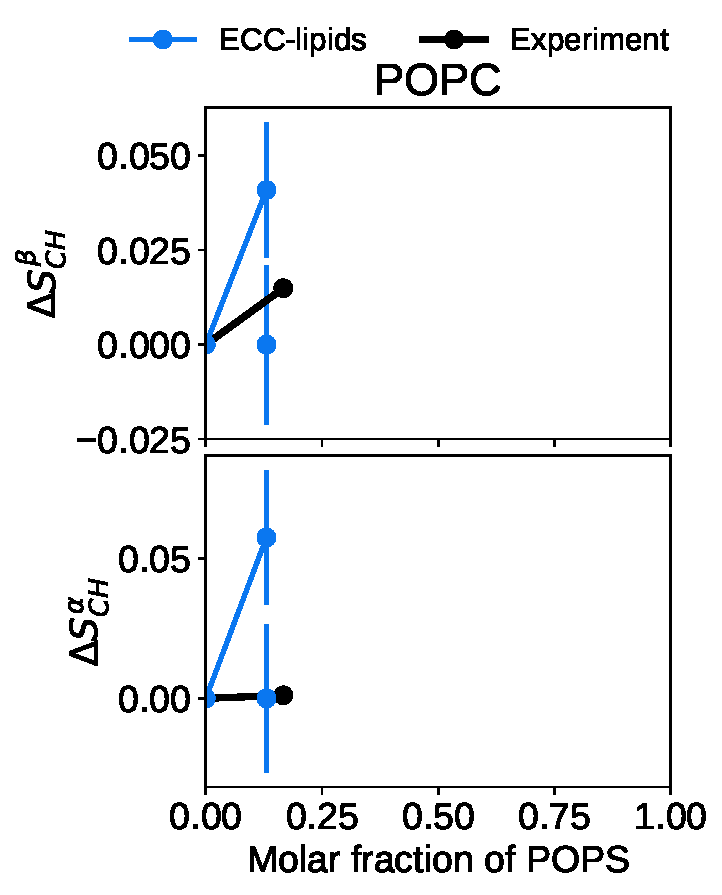
\includegraphics[width=\figwidth]{../img/ecc_pops/l17/order_parameters_changes_A-B_PC-PS_mix_POPC_nacl.pdf} 
  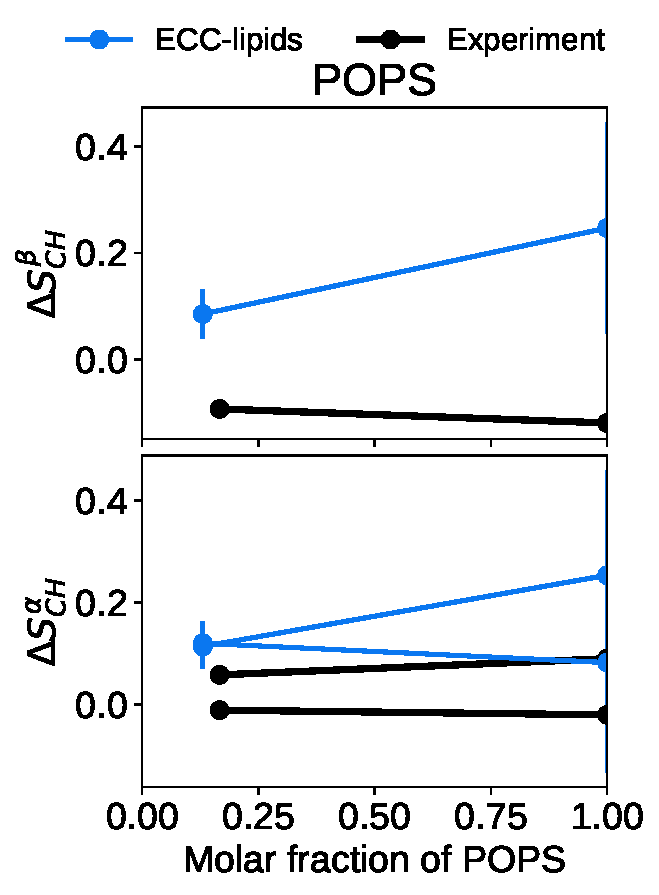
\includegraphics[width=\figwidth]{../img/ecc_pops/l17/order_parameters_changes_A-B_PC-PS_mix_POPS_nacl.pdf} 
  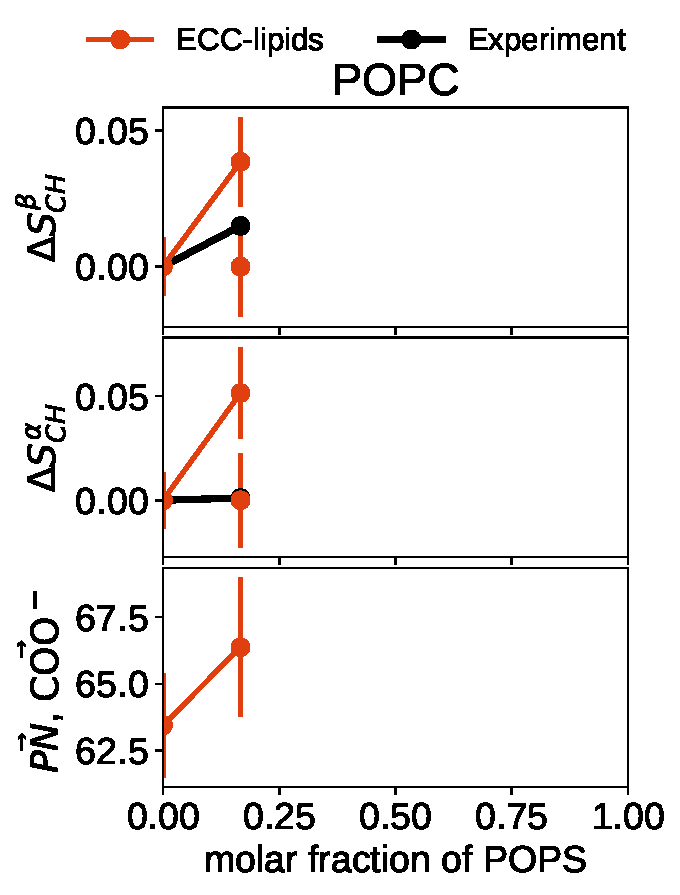
\includegraphics[width=\figwidth]{../img/ecc_pops/order_parameters_changes_A-B_PC-PS_mix_POPC_nacl.pdf} 
  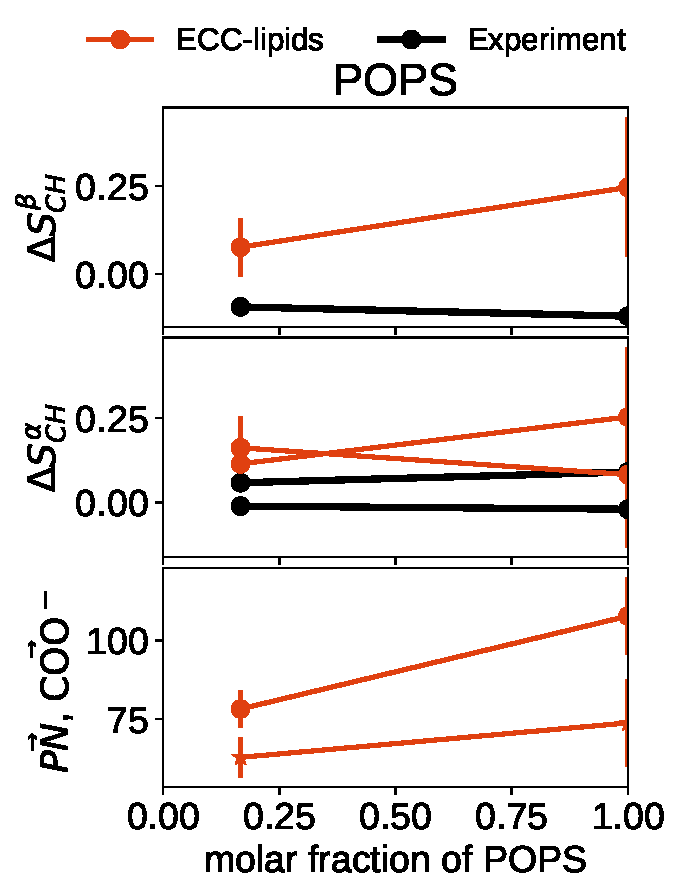
\includegraphics[width=\figwidth]{../img/ecc_pops/order_parameters_changes_A-B_PC-PS_mix_POPS_nacl.pdf} 
  \caption{\label{fig:delta_ordPar_NaCl_PC-PS_mix} 
    Changes of the head group order parameters of a POPC:POPS 5:1 bilayer as a function of PS content.
    Experimental points have inherent systematic error, as they come from different experiments.
    A complete series of points can be found (?) in \cite{roux90} -- which is to be added to the plot.
  } 
\end{figure} 
 
